% INTRODUÇÃO-------------------------------------------------------------------

%Coisas para perguntar: Seção sobre métricas;pessoa e tempo verbal de escrita;estado da arte;Cap de conceitos poderia ser o cap de Revisao de Literatura;
%TODO Capítulo de conceitos! (estado da arte)(extratores de características)(espaços métricos)(funções de distância)(estruturas de indexação)
%TODO Capítulo técnica omni
%TODO Retirar estado da arte da intro --> colocar em conceitos
%TODO Melhorar introdução Omni

\chapter{INTRODUÇÃO}
\label{chap:introducao}

Neste capítulo será apresentado uma contextualização do problema, assim como o estado da arte abordado por este trabalho.
Também será introduzido um tipo de consulta não-nativo ao SGBDR, a consulta por similaridade, assim como os tipos de consultas por similaridade
que serão utilizados neste trabalho como a consulta por abrangência e a consulta por k-vizinhos mais próximos. Finalmente, será apresentado a
organização deste documento.

\section{CONSIDERAÇÕES INICIAIS}
\label{sec:considini}

Nos anos recentes, foi notado um grande aumento no tráfego e armazenamento de diferentes aplicações e dados multimídias, como imagens, áudio, vídeo, impressões digitais, séries temporais,
sequências de proteínas, etc. Estes tipos de dados, que apresentam muito mais atributos do que simples numerais ou pequenas cadeias de caracteres, são conhecidos como dados complexos \cite{Zighed2008}.\par
Quando tratados por um Sistema Gerenciador de Banco de Dados Relacional (SGBDR), não suportam comparações com os operadores conhecidos como "big six"\ da linguagem SQL: $=$, $\neq$ , $<$, $>$, $\leq$, $\geq$.
Esse fato limita muito as comparações entre dados complexos inseridos em um SGBDR, ocasionando um grande problema no contexto de base de dados, uma vez que os principais sistemas de gerenciamento
de base de dados são relacionais \cite{DBE2017}. Com isso, tornou-se necessária a concepção de novos tipos de comparadores, como buscas por similaridade.\par 

Estas consultas por similaridade se aplicam de maneira geral a muitos dos tipos de dados complexos \cite{Barioni2009}. Embora equiparar duas imagens médicas (como tomografias de pacientes distintos) 
raramente produza um resultado diferente de falso, procurar por imagens semelhantes à original faz mais sentido e retorna resultados mais relevantes.

\section{TIPOS DE CONSULTAS}
\label{sec:tiposconsultas}

Dentre os operadores de consulta por similaridade os mais comuns são as consultas por abrangência (\textit{range query: Rq}) e consulta aos k-vizinhos mais próximos (\textit{k-nearest neighbor querry: kNNq}).\par 

As consultas por abrangência \textit{Rq($s_q$, $\xi$)} recebem como parâmetro um elemento $s_q$ do domínio de dados (elemento central da consulta) e um limite máximo de dissimilaridade $\xi$. O resultado é o conjunto de 
elementos da base que diferem do elemento central da consulta por no máximo a dissimilaridade indicada.\par
\begin{mydef}
 \label{def:def_rq}
  Seja $S$ um atributo complexo de um domínio $\mathbb{S}$ sobre o qual a condição de similaridade é expressada, seja $d$ uma
  função de distância, seja $\xi$ o limiar de dissimilaridade e seja $s_q \in \mathbb{S}$ o elemento central de consulta. 
  A consulta Rq($s_q$ , $\xi$) retorna todos os elementos $s_i \in \mathbb{S}$ que possuem o valor do atributo $S$ distantes
  até um máximo de $\xi$ deste atributo referente ao elemento central da consulta: 
  \begin{equation} \label{eq:knnq}   
    Rq(s_q, \xi): S = \{s_i \in S \ |\ d(s_i(S), s_q) \leq \xi\}
  \end{equation}
\end{mydef}

\begin{figure}[H]
\centering
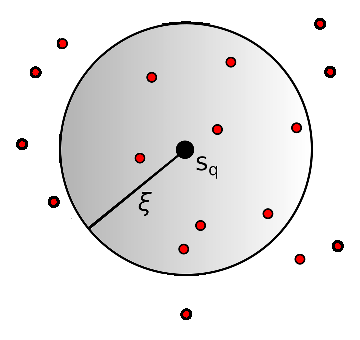
\includegraphics[width=.3\textwidth]{dados/figuras/rqu.eps}
\caption{Exemplo de consulta por abrangência}
\fonte{Autoria Própria}
\label{fig:exemplorq}
\end{figure}

A figura \ref{fig:exemplorq} exemplifica este tipo de consulta. Tomando $s_q$ e $\xi$ como parâmetros da consulta, todos os
elementos contidos pelo raio de abrangência fazem parte do conjunto resposta da consulta. $s_q$ não necessariamente precisa
pertencer ao conjunto de dados de pesquisa, devendo apenas pertencer ao mesmo domínio de dados.


Uma consulta aos k-vizinhos mais próximos \textit{kNNq($s_q$, $k$)} também recebe como um de seus parâmetros um elemento central da consulta $s_q$, e um número inteiro $k$ de vizinhos desejados, e retorna
como resultado o conjunto dos $k$ elementos com a menor dissimilaridade em relação ao elemento central da consulta $s_q$ \cite{POLA2010}.

\begin{mydef}
  \label{def:def_knnq}
  Seja $S$ um atributo complexo de um domínio $\mathbb{S}$ sobre o qual a condição de similaridade é expressada, seja $d$ uma
  função de distância, seja $k \in \mathbb{N^*}$ a quantidade de elementos desejados e seja $s_q \in \mathbb{S}$ o elemento
  central de consulta. A consulta kNNq($s_q$ , $k$) retorna $k$ elementos $s_i \in \mathbb{S}$ que possuem o valor do atributo $S$ menos distantes do valor 
  deste atributo referente ao elemento central da consulta\cite{Ferreira2009}:
  \begin{equation} \label{eq:knnq}   
    kNNq(s_q, k): S = \{s_i \in S \ |\  \forall \ s_j \in S - S^{'}, d(s_i, s_q)\leq d(s_j, s_q)\},
  \end{equation}
  onde $S^{'}$ = 0, se i = 1 e $S^{'}$ = \{$s_1$, ....., $s_{(i-1)}$\}, se 1 < i $\leq$ k. 
\end{mydef}

A figura \ref{fig:exemploknnq} exemplifica este tipo de operação. Nesta consulta, os parâmetros foram o elemento central da consulta $s_q$ e o número de elementos $k$ a serem
encontrados igual a 4. Os elementos ligados ao elemento central foram os mais próximos a este, portanto apenas eles fazem parte do conjunto resposta da consulta.
\begin{figure}[H]
\centering
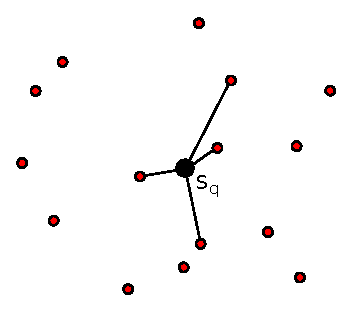
\includegraphics[width=.3\textwidth]{dados/figuras/knnq.eps}
\caption{Exemplo de consulta por k-vizinhos mais próximos}
\label{fig:exemploknnq}
\fonte{Autoria Própria}
\end{figure}

O SGBDR não possui suporte nativo a estes tipos de consulta, mas é possível construir estas consultas utilizando ferramentas existentes em um banco de dados relacional (como a \textit{B-tree}).\par %escopo do trabalho

A solução abordada por esta proposta é a do uso de técnicas Omni, presentes no trabalho de \cite{Traina2001}. Um número calculado de elementos do conjunto de dados são selecionados como "focos", e utilizados para
podar cálculos desnecessários de distâncias, fazendo uso da desigualdade triangular. 

A base da técnica Omni é calcular previamente as distâncias de todos os elementos para todos os focos selecionados, armazenando estas distâncias no banco. Quando uma consulta por similaridade
(como uma consulta por abrangência) é realizada, são conhecidas as distâncias entre o elemento central da consulta $s_q$ e o raio de abrangência $\xi$. Considerando um foco ${f_1}$ e utilizando
a desigualdade triangular, elementos que possuem uma distância entre o foco escolhido menor do que a distância de $s_q$ até o foco menos o valor $\xi$ serão descartados do conjunto de elementos necessários para
os cálculos de distância com o elemento central. Simetricamente, elementos cuja distância até o foco seja maior do que a distância de $s_q$ até o foco mais o valor do raio de abrangência $\xi$ também
serão descartados. Com isso, ocorre uma grande redução do número de cálculos necessários para fornecer o conjunto resposta. Essa poda também pode ser realizada por mais de um foco.

\begin{figure}[H]
\centering
\caption{Consulta por abrangência pela técnica Omni utilizando um foco}
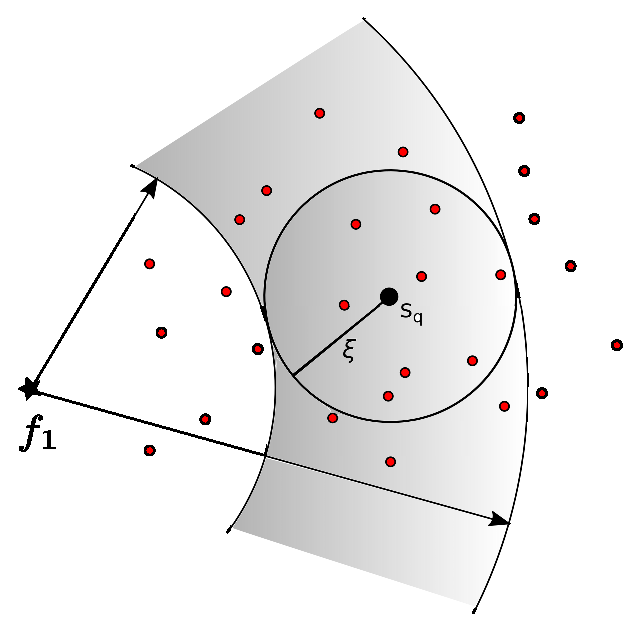
\includegraphics[width=.4\textwidth]{dados/figuras/rg_omni_1.eps}
\fonte{Autoria Própria}
\label{fig:rqomni1}
\end{figure}


A figura \ref{fig:rqomni1} ilustra a poda no número de cálculos. Apenas os elementos na área sombreada terão as suas distâncias em relação ao centro da consulta calculadas, pois estão no
conjunto de elementos que não foram descartados utilizando a desigualdade triangular com as distâncias previamente calculadas em relação ao foco. O armazenamento das distâncias de cada foco ${f_i}$ para cada outro elemento $s_k$ será feito 
utilizando uma estrutura de indexação que implementa os conceitos da técnica Omni com a estrutura da B$^+$-tree, originando uma nova estrutura chamada de Omni-Btree. As distâncias serão armazenadas em $l$ Omni-Btrees, sendo $l$ o número de focos
criados para a base de dados \cite{Traina2001}.

\section{OBJETIVOS}
\label{sec:objetivos}
Os objetivos encontram-se divididos em objetivos gerais, referentes ao resultado obtido com a conclusão deste trabalho e objetivos específicos, ilustrando etapas intermediárias necessárias para alcançar o objetivo geral.
\subsection{OBJETIVOS GERAIS}
\label{subsec:objger}
O principal foco deste trabalho é a construção de um sistema de consultas por similaridade em uma base de imagens utilizando técnicas da família Omni para reduzir o custo computacional das operações de consulta.

\subsection{OBJETIVOS ESPECÍFICOS}
\label{subsec:objesp}
\begin{itemize}
 \item Modelar o banco de dados para atender a problemática apresentada;
 \item Aplicar os extratores de características das imagens utilizadas;
 \item Povoar o banco de dados com as imagens e os valores de suas características; %inserir a base de imagens
 \item Criar a estrutura Omni necessária para a filtragem dos cálculos;
 \item Analisar e comparar os resultados obtidos.
\end{itemize}


\section{ORGANIZAÇÃO DO TRABALHO} %TODO Melhorar isso
\label{sec:organizacaoTrabalho}

A estrutura deste trabalho apresenta mais detalhes sobre os tipos de consulta por similaridade utilizados, assim como os seus algoritmos computacionais. Posteriormente, explana os conceitos e técnicas da família Omni utilizada para
melhorar a performance das consultas. Também realiza a abordagem sobre os extratores de características utilizados para a base de imagens utilizada neste trabalho.
